\documentclass[10pt]{article}

\usepackage{fullpage}
\usepackage{graphics}
\usepackage{natbib}
\usepackage{amssymb,amsthm,amsmath}

\newtheorem{proposition}{Proposition}
\newtheorem{lemma}[proposition]{Lemma}
\newtheorem{corollary}[proposition]{Corollary}
\newtheorem{theorem}[proposition]{Theorem}

\newcommand{\R}{\mathbb{R}}

\renewcommand{\P}{\mathcal{P}}
\newcommand{\U}{\mathcal{U}}
\newcommand{\X}{\mathcal{X}}
\newcommand{\indicator}[1]{\mathbf{1}\left[{#1}\right]}
\newcommand{\x}{\mathbf{x}}
\newcommand{\KL}[2]{D\left(#1 \middle\| #2 \right)}
\newcommand{\norm}[1]{\left\| #1 \right\|}

\DeclareMathOperator{\argmin}{argmin}
\DeclareMathOperator{\err}{err}
\DeclareMathOperator{\Exp}{\mathbf{E}}
\DeclareMathOperator{\VC}{VC}

\begin{document}

\title{The information-theoretic value of unlabeled data in semi-supervised learning}
\author{Alexander Golovnev \and D\'avid P\'al \and Bal\'azs Sz\"or\'enyi}

\maketitle

\begin{abstract}
We show a separation of the number of labeled examples required between learning \emph{with}
and \emph{without} the knowledge of the distribution of the unlabeled data. For
the class of projections over the Boolean hypercube of dimension $n$, we show a
separation by $\Theta(\frac{\log n}{\log \log n})$ multiplicative factor.

Learning with the knowledge of the distribution (a.k.a. \emph{fixed-distribution
learning}) can be viewed as an idealized scenario of semi-supervised learning
where the number of unlabeled data points is so great that the unlabeled
distribution is known exactly. For this reason, we call the separation
the \emph{value of unlabeled data}.
\end{abstract}


\section{Introduction}

\cite{Hanneke-2016} showed that for any class $C$ of Vapnik-Chervonenkis
dimension $d$ there exists an algorithm that $\epsilon$-learns any target
function from $C$ under any distribution from $O\left(\frac{d +
\log(1/\delta)}{\epsilon}\right)$ labeled examples with probability at least
$1-\delta$. \cite{Benedek-Itai-1991} showed that for any class $C$ and any
distribution there exists an algorithm that $\epsilon$-learns any target from
$C$ from $O \left( \frac{\log N_\epsilon + \log (1/\delta)}{\epsilon}\right)$ labeled
examples with probability at least $1-\delta$ where $N_\epsilon$ is the size of an
$\epsilon$-covering of $C$ with respect to the disagreement metric $d(f,g) =
\Pr[f(x) \neq g(x)]$. Ignoring $\log(1/\epsilon)$ factor, Benedek-Itai bound
is never worse than Hanneke's bound, since $N_\epsilon = O(1/\epsilon)^{O(d)}$; see
\cite{Dudley-1978}.

Benedek-Itai's algorithm receives as input the distribution of unlabeled data.
(The algorithm uses it to construct the $\epsilon$-cover.) Unsurprisingly, there
exist distributions for which Benedek-Itai's bound on the sample complexity is
significantly lower then the Hanneke's bound. For instance, a distribution with
support on a single point has cover of size $2$. That leaves the possibility
that there exists an algorithm that does \emph{not} depend on the distribution
and achieves Benedek-Itai bound (or a slightly worse bound) for \emph{every}
distribution. In fact, one would think that empirical risk minimization (ERM) or
Hanneke's algorithm could be such algorithm. There is reason good to think that:
ERM needs significantly less labeled examples to learn any target under some
unlabeled distributions, e.g. for distributions concentrated on a single point
ERM needs only one labeled example. If ERM, Hanneke's algorithm, or some other
distribution-independent algorithm had sample complexity that matches (or nearly
matches) the optimal distribution-specific sample complexity for \emph{every}
distribution, we could conclude that the knowledge of unlabeled data
distribution is completely useless.

As \cite{Darnstadt-Simon-Szorenyi-2013} showed this not the case. They showed
that any algorithm for learning projections over $\{0,1\}^n$ that does not
depend on the unlabeled data, requires, for some data distributions, more
labeled examples than the Benedek-Itai bound. However, they did not quantify
this gap, beside stating that it grows without bound as $n$ goes to infinity.
In this paper, we quantify the gap by showing that \emph{any}
distribution-independent algorithm for learning the class of projections over
$\{0,1\}^n$ requires, for some unlabeled distributions, $\Omega(\frac{\log
n}{\log \log n})$ times as many labeled examples as Benedek-Itai bound.

\section{Related Work}

The question of whether knowledge of unlabeled data distribution helps was
proposed and initially studied by \cite{Ben-David-Lu-Pal-2008}. However, their
paper considers only classes with Vapnik-Chervonenkis dimension at most $1$
or distributions where the size of the covering is
$\Theta(1/\epsilon)^{\Theta(\VC(C))}$ i.e. as large as it can be.\footnote{For
any concept class and any distribution, the size of the smallest
$\epsilon$-cover is at most $O(1/\epsilon)^{O(\VC(C))}$.} In these settings,
separation does not exist and they (incorrectly) concluded that unlabeled data
are useless.

The question was studied in earnest by \cite{Darnstadt-Simon-Szorenyi-2013} who
show two major results. First, they show that for any concept class $C$ and for
every distribution the ratio of the sample complexities between
distribution-independent and distribution-dependent algorithms is at most
$\VC(C)$. Second, they show that for the class of projections over $\{0,1\}^n$,
there are distributions where the ratio grows to infinity as a function of $n$.

In learning theory, the disagreement metric and $\epsilon$-cover was  introduced
by \cite{Benedek-Itai-1991} but the ideas are much older; see
e.g.~\cite{Dudley-1978, Dudley-1984}. The $O(1/\epsilon)^{O(\VC(C))}$ upper
bound on size of the smallest $\epsilon$-cover is by \citet[Lemma
7.13]{Dudley-1978}; see also \citet[Chapter 4]{Devroye-Lugosi-2000} and
\cite{Haussler-1995}.

For any distribution-independent algorithm and any class $C$ of
Vapnik-Chervonenkis dimension $d \ge 2$ and any $\epsilon \in (0,1)$ and $\delta
\in (0,1)$ there exists a distribution over the domain and a concept which
requires at least $\Omega \left(\frac{d + \log(1/\delta)}{\epsilon}\right)$
examples to $\epsilon$-learn with probability at least $1 - \delta$;
see~\cite[Theorem 5.3]{Anthony-Bartlett-1999} and
\cite{Blumer-Ehrenfeucht-Haussler-Warmuth-1989,
Ehrenfeucht-Haussler-Kearns-Valiant-1989}. The proof of the lower bound
constructs a distribution that does \emph{not} depend on the algorithm. The
distribution is a particular distribution over a fixed set shattered by $C$. So
even an algorithm that knows the distribution requires $\Omega \left(\frac{d +
\log(1/\delta)}{\epsilon}\right)$ to learn.

To better understand the relationship of the upper and lower bounds, we
summarize the situation for the class of projections over $\{0,1\}^n$ in
Figure~\ref{figure:sample-complexity}. Recall that Vapnik-Chervonenkis dimension
of projections over $\{0,1\}^n$ is $\lfloor \log_2 n \rfloor$. This is a
folklore result, which we re-prove as
Proposition~\ref{proposition:vc-dimension-projections}.

\begin{figure}
\centering
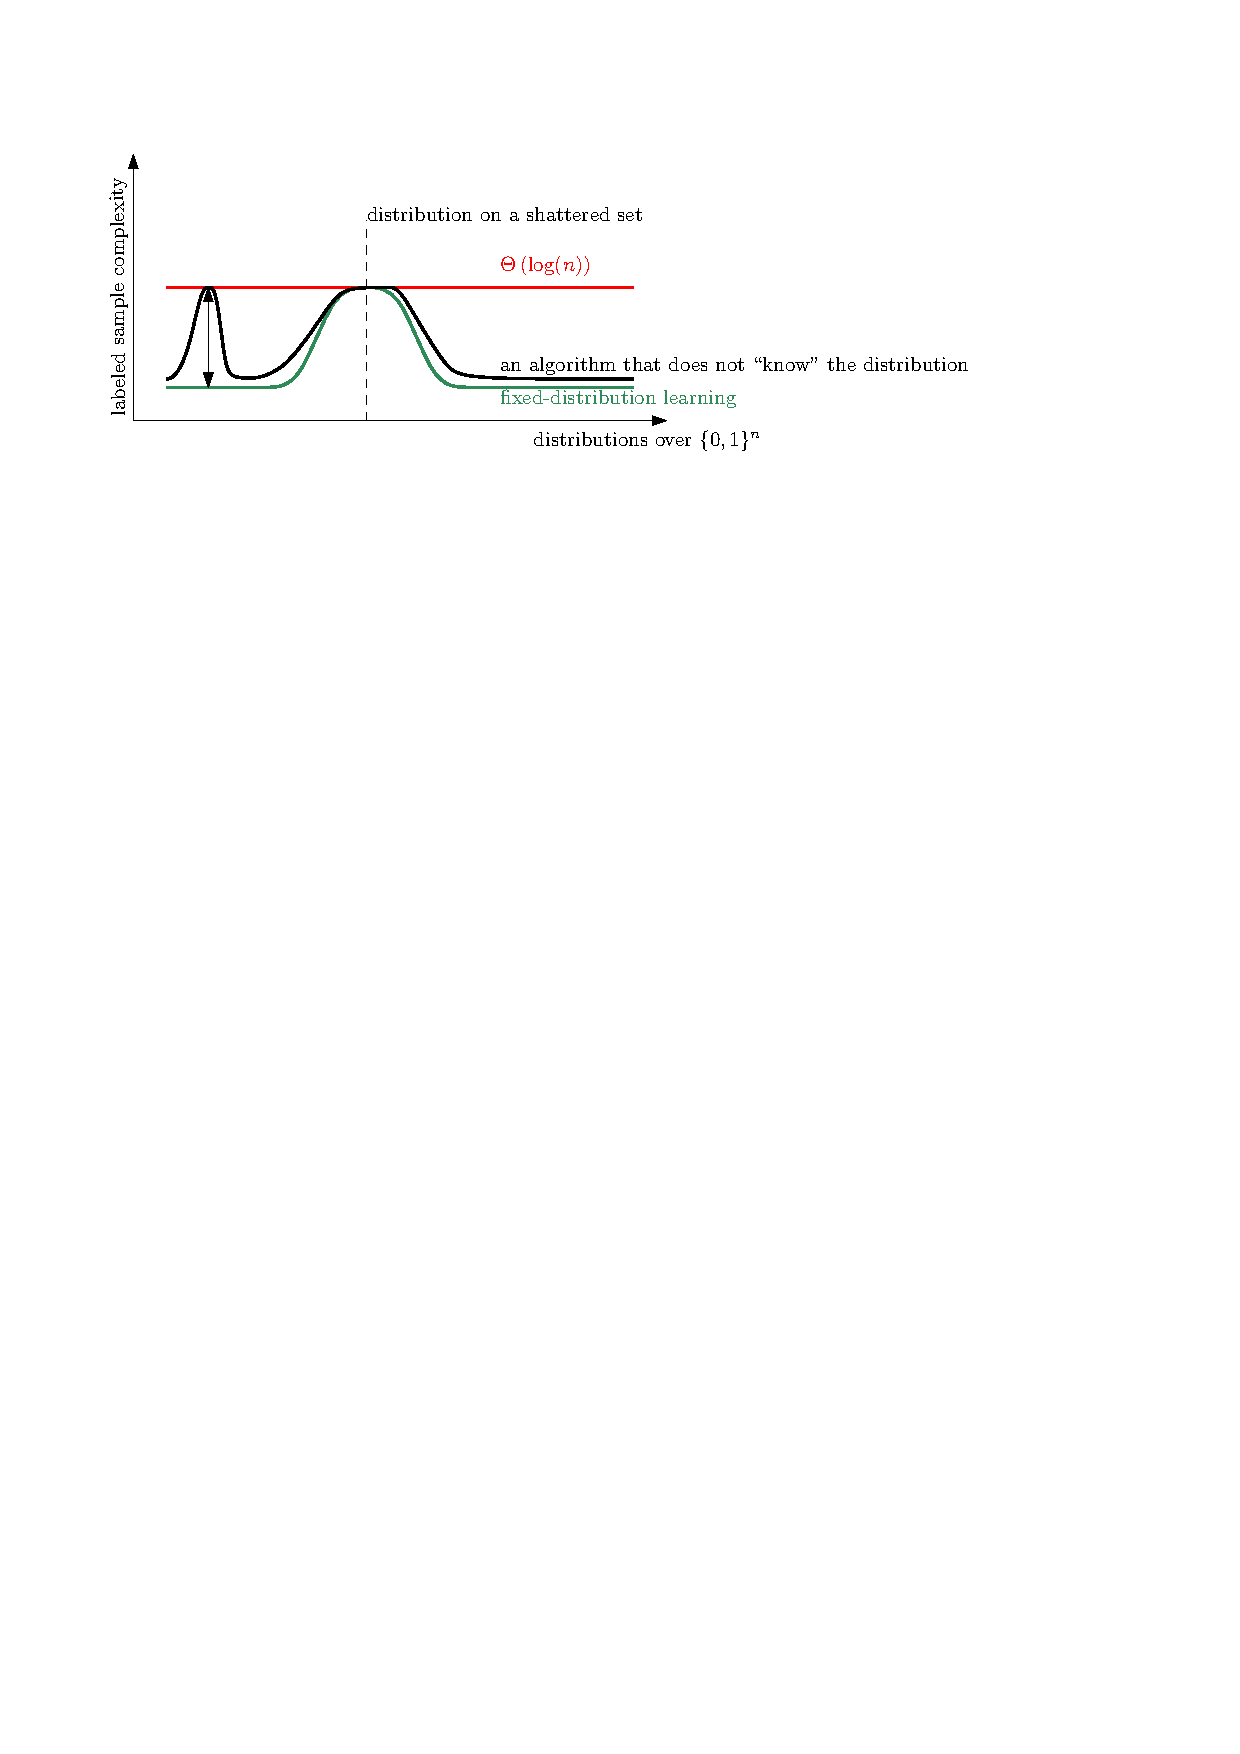
\includegraphics{figure}
\caption{The graph shows sample complexity bounds of learning a class of
projections over the domain $\{0,1\}^n$ under various unlabeled distributions.
We assume that $\epsilon$ and $\delta$ are constant, say, $\epsilon = \delta =
\frac{1}{10}$. The graph shows three lines. The red horizontal line is the
optimal Hanneke's bound for the class of projections, which is
$\Theta(\VC(C_n)) = \Theta(\log n)$. The green line corresponds to to
Benedek-Itai bound. The green line touches the red line for certain
distributions, but is lower for other distributions. In particular, for certain
distributions the green line is $O(1)$. The dashed line corresponds
to a particular distribution on a shattered set. This is where the green line
and red line touch. Furthermore, here the the upper bound coincide
with the lower bound for that particular distribution.
The black line is the sample complexity
of an arbitrary \emph{distribution-independent} algorithm. (For example, the
reader can think of the ERM or Hanneke's algorithm.) Obviously, the black line
must lie above the green line. We prove that there exist a distribution where
the black line is $\Omega(\frac{\log n}{\log \log n})$ times higher than the
green line.} \label{figure:sample-complexity}
\end{figure}

\section{Preliminaries}

Let $\X$ be a non-empty set. We denote by $\{0,1\}^\X$ the class of all
functions from $\X$ to $\{0,1\}$. A \emph{concept class over a domain $\X$} is a
subset $C \subseteq \{0,1\}^\X$. A \emph{labeled example} is a pair $(x,y) \in
\X \times \{0,1\}$.

A \emph{distribution-independent learning algorithm} is a function
$A:\bigcup_{m=0}^\infty \left(\X \times \{0,1\} \right)^m \to \{0,1\}^\X$. In
other words, the algorithm gets as input a sequence of labeled examples $(x_1,
y_1), (x_2, y_2), \dots, (x_m, y_m)$ and outputs a function from $\X$ to
$\{0,1\}$. We allow the algorithm to output function that does not belong to
$C$, i.e., the algorithm can be improper. A \emph{distribution-dependent algorithm}
is a function that maps any probability distribution over $\X$ to a
distribution-independent algorithm.

Let $P$ be a probability distribution over a domain $\X$. For any two functions
$f:\X \to \{0,1\}$, $g:\X \to \{0,1\}$ we define the disagreement pseudo-metric
$$
d_P(f,g) = \Pr_{X \sim P}[f(X) \neq g(X)] \; .
$$
Let $C$ be concept class over $\X$, let $c \in C$, let $\epsilon, \delta \in (0,1)$.
Let  $X_1, X_2, \dots, X_m$ be an i.i.d. sample from $P$. We define the corresponding
labeled sample $T = ((X_1, c(X_1)), (X_2, c(X_2)), \dots, (X_m, c(X_m)))$.
We say that an algorithm $A$, \emph{$\epsilon$-learns} target $c$ from $m$ samples
with probability at least $1 - \delta$ if
$$
\Pr \left[d_P(c,A(T)) \le \epsilon \right]  \ge 1 - \delta \; .
$$

Below we state two simple propositions that are useful for proving lower bounds
on the number of labeled samples. The first proposition says that if average
error $d_P(c,A(T))$ is high, the algorithm can't $\epsilon$-learn. The second
proposition says that the best algorithm for predicting a bit computes
conditional expectation of the bit and thresholds it at $1/2$.

\begin{proposition}[Error probability vs. Expected error]
\label{proposition:error-probability-vs-expected-error}
Let $Z$ be a random variable such that $Z \le 1$ with probability one.
Then,
$$
\Pr[Z > \epsilon] \ge \frac{\Exp[Z] - \epsilon}{1 - \epsilon} \qquad \text{for any $\epsilon \in [0, 1)$.}
$$
\end{proposition}

\begin{proof}
We have
$$
\Exp[Z]
\le \epsilon \cdot \Pr[Z \le \epsilon] + 1 \cdot \Pr[Z > \epsilon]
= \epsilon \cdot (1 - \Pr[Z > \epsilon]) + \Pr[Z > \epsilon] \; .  \qquad \qedhere
$$
Solving for $\Pr[Z > \epsilon]$ finishes the proof.
\end{proof}

\begin{proposition}[Optimality of Bayes Predictor]
\label{proposition:bayes}
Let $\U$ be a finite set. Let $U,V$ be a random variables such that $U \in \U$ and $V \in \{0,1\}$ with probability one.
Let $f:\U \to \{0,1\}$ be a predictor. Then,
$$
\Pr\left[ f(U) \neq V \right]
\ge \sum_{u \in \U} \left( \frac{1}{2} - \left| \frac{1}{2} -  \Exp \left[V \, \middle| \, U = u\right] \right| \right) \cdot \Pr[U = u] \; .
$$
\end{proposition}

\begin{proof}
We have
$$
\Pr \left[ f(U) \neq V \right] = \sum_{u \in \U} \Pr \left[ f(U) \neq V \, \middle| \, U = u \right] \cdot \Pr[U = u] \; .
$$
It remains to show that
$$
\Pr\left[ f(U) \neq V \, \middle| \, U = u \right]
\ge
\frac{1}{2} - \left| \frac{1}{2} -  \Exp \left[V \, \middle| \, U = u \right] \right| \; .
$$
Since if  $U=u$, the value $f(U) = f(u)$ is fixed, and hence
\begin{align*}
\Pr\left[ f(U) \neq V \, \middle| \, U = u \right]
& \ge \min\left\{ \Pr \left[ V = 1 \, \middle| \, U = u \right], \ \Pr \left[ V = 0 \, \middle| \, U = u \right] \right\} \\
& = \min\left\{ \Exp \left[ V  \, \middle| \, U = u \right], \ 1 - \Exp \left[ V \, \middle| \, U = u \right] \right\} \\
& = \frac{1}{2} - \left| \frac{1}{2} -  \Exp \left[ V  \, \middle| \, U = u \right] \right|
\end{align*}
We used the fact that $\min\{x, 1 - x\} = \frac{1}{2} - \left| \frac{1}{2} - x \right|$ for all $x \in \R$
which can be easily verified by considering two cases: $x \ge \frac{1}{2}$ and $x < \frac{1}{2}$.
\end{proof}

\begin{theorem}[Chernoff-Hoeffding bound]
Let $X_1, X_2, \dots, X_n$ be i.i.d. Bernoulli variables with parameter $p$.
Then, for any $\epsilon \ge 0$,
$$
\Pr \left[{\frac {1}{n}} \sum_{i=1}^n X_i \ge p + \epsilon \right] \le e^{ - 2n \epsilon^2}  \qquad \text{and} \qquad
\Pr \left[{\frac {1}{n}} \sum_{i=1}^n X_i \le p - \epsilon \right] \le e^{ - 2n \epsilon^2}  \; . \\
$$
\end{theorem}

\section{Projections}

We denote by $C_n$ the class of \emph{projections} over the domain $\X = \{0,1\}^n$. The
class $C_n$ consists of $n$ functions $c_1, c_2, \dots, c_n$ from $\{0,1\}^n$ to
$\{0,1\}$. For any $i \in \{1,2,\dots,n\}$, for any $x \in \{0,1\}^n$,
the function $c_i$ is defined as $c_i((x[1], x[2], \dots, x[n])) = x[i]$.

For any $p \in (0,\frac{1}{4})$ and $n \ge 2$,
we consider a family $\P_{n,p}$ consisting of
$n$ probability distributions $P_1, P_2, \dots, P_n$ over the Boolean hypercube
$\{0,1\}^n$. In order to describe the distribution $P_i$, for some $i$, let $X =
(X[1], X[2], \dots, X[n])$ be a random vector drawn from $P_i$. The distribution
$\P_i$ is a product distribution, i.e., $\Pr[X = x] = \prod_{j=1}^n \Pr[X[j] =
x[j]]$ for any $x \in \{0,1\}^n$. The marginal distributions of the coordinates
are
$$
\Pr[X[j] = 1] =
\begin{cases}
\frac{1}{2} & \text{if $j = i$,} \\
p & \text{if $j\neq i$.} \\
\end{cases}
$$
Throughtout the paper we treat $p$ as a constant that does not depend
on $n$. The reader can think of $p=1/100$.

\begin{proposition}
\label{proposition:vc-dimension-projections}
Vapnik-Chervonenkis dimension of $C_n$ is $\lfloor \log_2 n \rfloor$.
\end{proposition}

\begin{proof}
Let us denote the Vapnik-Chervonenkis dimension by $d$. Recall that $d$ is the
size of the largest shattered set. Let $S$ be any shattered set of size $d$.
Then, there must be at least $2^d$ distinct functions in $C_n$. Hence, $d \le
\log_2 |C_n| = \log_2 n$. Since $d$ is an integer, we conclude that $d \le
\lfloor \log_2 n \rfloor$.

On the other hand, we construct a shattered set of size $\lfloor \log_2 n
\rfloor$. The set will consists of points $x_1, x_2, \dots, x_{\lfloor \log_2 n
\rfloor} \in \{0,1\}^n$. For any $i \in \{1,2,\dots,\lfloor \log_2 n \rfloor\}$
and any $j \in \{0,1,2,\dots,n-1\}$, we define $x_i[j]$ to be the $i$-th bit of the
in the binary representation of the number $j$. (The bit at position $i=1$ is the
least significant bit.) It is not hard to see that for any $v \in
\{0,1\}^{\lfloor \log_2 n \rfloor}$, there exists $c \in C_n$ such that $v =
(c(x_1), c(x_2), \dots, c(x_{\lfloor \log_2 n \rfloor}))$. Indeed, given $v$,
let $k \in \{0,1,\dots,2^{\lfloor \log_2 n \rfloor} - 1\}$ be the number with
binary representation $v$, then we can take $c = c_{k+1}$.
\end{proof}


\begin{theorem}[Lerning with knowledge of the distribution]
For any $n \ge 2$, there exists a distribution-dependent algorithm such that
for any $p \in (0,\frac{1}{4})$, any distribution from $\P_{n,p}$, any $\delta
\in (0,1)$, any target function $c \in C_n$, such that the algorithm
$2p$-learns the target using $O \left( \log(1/\delta) \right)$
labeled examples with probability at least $1 - \delta$.
\end{theorem}

\begin{proof}
Given a distribution $P_i \in \P_{n,p}$ for some $i \in \{1,2,\dots,n\}$, the
algorithm chooses two candidate functions $c_i, c_j \in C_n$ where $j$ is
arbitary index in $\{1,2,\dots,n\} \setminus \{j\}$. Given a sample $T =
((x_1, y_1), (x_2, y_2), \dots, (x_m,y_m))$ it outputs either $c_i$ or $c_j$
depending on which one has smaller empirical error. Recall that
empirical error of a classifier $h:\X \to \{0,1\}$ is
$$
\widehat \err(h) = \frac{1}{m} \sum_{t=1}^m \indicator{y_t \neq h(x_t)} \; .
$$
If $x_1, x_2, \dots, x_m$ are drawn i.i.d. from $P_i$
and the target function is $c_k \in C_n$ then
$\Exp[\widehat \err(h)] = d_{P_i}(c_k, h)$.

There are three cases. Either $k = i$, $k = j$ or $k \not \in {i,k}$.

\emph{Case $k=i$} In this case $\widehat \err(c_i) = 0$ with probability one.
Since $\indicator{y_t \neq c_j(x_t)}$ is a Bernoulli variable with parameter
$d_{P_i}(c_k, c_j) = d_{P_i}(c_i, c_j) = \frac{1}{2}$. Thus,
using Chernoff-Heoffding bound with $\epsilon = \frac{1}{2}$,
$$
\Pr[\widehat \err(c_j) > \widehat \err(c_i)] = \Pr[\widehat \err(c_j) > 0] \ge 1 - e^{m/2} \ge 1 - \delta \; .
$$
Therefore, with probability $1 - \delta$, the algorithm outputs the correct target $c_i$.

\emph{Case $k=j$} In this case $\widehat \err(c_j) = 0$ with probability one.
Since $\indicator{y_t \neq c_i(x_t)}$ is a Bernoulli variable with parameter
$d_{P_i}(c_k, c_i) = d_{P_i}(c_i, c_j) = \frac{1}{2}$. Thus,
using Chernoff-Heoffding bound with $\epsilon = \frac{1}{2}$,
$$
\Pr[\widehat \err(c_i) > \widehat \err(c_j)] = \Pr[\widehat \err(c_i) > 0] \ge 1 - e^{m/2} \ge 1 - \delta \; .
$$
Therefore, with probability $1 - \delta$, the algorithm the correct target $c_i$.


The proof relies on a result of \cite{Benedek-Itai-1991} for learning under
``fixed'' distributions. If $P$ is any probability distribution on some domain,
then $d_P(f,g) = \Pr_{X \sim P}[f(X) \neq g(X)]$ is a pseudo-metric on the set of all
$\{0,1\}$-valued functions on the domain. \cite{Benedek-Itai-1991} proved that
if a $C$ class of $\{0,1\}$-functions has an $\frac{\epsilon}{2}$-cover of size
$N$, then any target from $C$ is $\epsilon$-learnable from $O
\left( \frac{\log N + \log (1/\delta)}{\epsilon}\right)$ examples
with probability at least $1-\delta$.

For our purposes we pick $\epsilon = \frac{1}{5}$. We show that for any
distribution in $\P_n$ the class $C_n$ has an $\frac{1}{10}$-cover of size $N =
2$. This will imply the lemma.

Consider a distribution $P_i \in \P_{n,p}$ for some $i \in \{1,2,\dots,n\}$.
Pick any $j \in \{1,2,\dots,n\}$ such that $j \neq i$.
We claim that $C' = \{ c_i, c_j \}$ is an $\frac{1}{10}$-cover of
$C_n$. That is, we claim that for any $c \in C_n$, there exists $c' \in
C'$ such that $d_{P_{\sigma}}(c,c') \le \frac{1}{10}$.

Any $c \in C_n$ is of the form $c = c_k$. If $k \in \{i,j\}$ then, trivially, $c \in C'$ and $d_{P_i}(c,c) = 0$.
Otherwise, if  $k \not \in \{i,j\}$, let $p = \frac{1}{\ln n}$,
$$
d_{P_i}(c_j, c_k)
= \Pr_{X \sim P_i}[X_j \neq X_k] \\
= 2 p (1 - p) \\
\le 2p \; .
$$
\end{proof}



\begin{theorem}[Learning without knowledge of the distribution]
For any algorithm $A$ there exists a distribution $P \in \P_n$ and a target
concept $c \in C_n$ such that the algorithm requires at least  $\Omega \left(
\frac{\log n}{\log \log n} \right)$ labeled examples to $\frac{1}{10}$-learn the
target concept with probability at least $\frac{5}{6}$.
\end{theorem}

\begin{proof}
Let $A$ be any learning algorithm. For ease of notation, we formalize it is as a function
$$
A:\bigcup_{m=0}^\infty \left(\{0,1\}^{m \times n} \times \{0,1\}^m\right) \to \{0,1\}^{\{0,1\}^n} \; .
$$
The algorithm receives an $m \times n$ matrix and a binary vector of length $m$.
The rows of the matrix corresponds to unlabeled examples and the vector encodes
the labels. The output of the $A$ is any function from $\{0,1\}^n \to \{0,1\}$.

Let $n \ge 8$. Fix the number of examples $m$ to be any non-negative integer less than
$\frac{\ln n}{3 \ln \ln n}$. We demonstrate the existence of a pair $(P,c) \in
\P_n \times C_n$ by probabilistic method.

Let $I$ be chosen uniformly at from $\{1,2,\dots,n\}$. We consider distribution $P_I \in \P_n$ and target $c_I \in C_n$.
Let $X_1, X_2, \dots, X_m$ be an i.i.d. sample from $P_I$ and
let $Y_1 = c_I(X_1), Y_2 = c_I(X_2), \dots, Y_m = c_I(X_m)$ be the target
labels. Let $X$ be $m \times n$ matrix with entries $X_i[j]$ and let $Y = (Y_1,
Y_2, \dots, Y_m)$ be the vector of labels. The output of the algorithm is $A(X,Y)$.
We will show that
\begin{equation}
\label{equation:failure-probability}
\Exp \left[d_{P_I}(c_I, A(X,Y)) \right] \ge \frac{1}{4} \; .
\end{equation}
This means that there exists $i \in \{1,2,\dots,n\}$ such that
$$
\Exp \left[d_{P_i}(c_i, A(X,Y)) \right] \ge \frac{1}{4}
$$
which, by Proposition~\ref{proposition:error-probability-vs-expected-error} with $\epsilon=1/10$, implies that
$$
\Pr \left[ d_{P_i}(c_i, A(X,Y)) \ge \frac{1}{10} \right] \ge \frac{\frac{1}{4} - \frac{1}{10}}{1 - \frac{1}{10}} = \frac{1}{6} \; .
$$

It remains to prove \eqref{equation:failure-probability}.
Let $Z$ be a test sample drawn from $P_I$. That is, conditioned on $I$, the sequence $X_1, X_2, \dots, X_m, Z$ is i.i.d. drawn from $P_I$.
Then, by Proposition~\ref{proposition:bayes},
\begin{align*}
& \Exp \left[d_{P_I}(c_I, A(X,Y))\right] \\
& = \Pr\left[ A(X,Y)(Z) \neq c_I(Z) \right] \\
& \ge \sum_{\substack{x \in \{0,1\}^{m \times n} \\ y \in \{0,1\}^m \\ z \in \{0,1\}^n}} \frac{1}{2} - \left| \frac{1}{2} - \Exp\left[ c_I(Z) \, \middle| \, X = x, Y = y, Z = z \right] \right| \cdot \Pr \left[X = x, Y = y, Z = z \right] \; .
\end{align*}
We need to compute $\Exp\left[ c_I(X_{m+1}) \, \middle| \, X = x, Y = y, Z = z \right]$.
For that we need some additional notation.
For any $x \in \{0,1\}^{m \times n}$, let $x[1], x[2], \dots, x[n]$ be its columns.
For any $x \in \{0,1\}^{m \times n}$ and $y \in \{0,1\}^m$ let
$$
k(x,y) = \{ i \in \{1,2,\dots,n\} ~:~ B[i] = y \}
$$
be the set of indices of columns matching the column of labels $y$. The key observation is due to symmetry, for $i = 1,2,\dots,n$,
\begin{align*}
\Pr \left[I = i \, \middle| \, X = x, Y = y \right]
=
\begin{cases}
\frac{1}{|k(x,y)|} & \text{if $i \in k(x,y)$,} \\
0 & \text{if $i \not \in k(x,y)$,} \\
\end{cases}
\end{align*}
Next, let
$$
p = \frac{1}{\ln n} \; .
$$
By definition of the distribution $P_I$ and that conditioned on $I$, the variables $X,Y,Z$ are independent,
we have for any $x \in \{0,1\}^n$, and $i = 1,2,\dots,n$,
\begin{align*}
\Pr \left[Z = z \, \middle| \, I = i, X = x, Y = y \right]
& = \Pr \left[Z = z \, \middle| \, I = i \right] \\
& =
\begin{cases}
\frac{1}{2} p^{\norm{z}_1 - 1} (1 - p)^{n - \norm{z}_1} & \text{if $z[i] = 1$,} \\
\frac{1}{2} p^{\norm{z}_1} (1-p)^{n-1 - \norm{z}_1}& \text{if $z[i] = 0$.} \\
\end{cases}
\end{align*}
This allows us to compute the conditional probability
\begin{align*}
& \Pr \left[I = i, Z = z \, \middle| \, X = x, Y = y \right] \\
& \quad = \Pr \left[Z = z \, \middle| \, I = i, X = x, Y = y \right] \cdot \Pr \left[I = i \, \middle| \, X = x, Y = y \right] \\
& \quad =
\begin{cases}
\frac{1}{2|k(x,y)|} p^{\norm{z}_1 - 1} (1 - p)^{n - \norm{z}_1} & \text{if $i \in k(x,y)$ and $z[i] = 1$,} \\
\frac{1}{2|k(x,y)|} p^{\norm{z}_1} (1 - p)^{n - 1 - \norm{z}_1} & \text{if $i \in k(x,y)$ and $z[i] = 0$,} \\
0 & \text{if $i \not \in k(B,y)$.} \\
\end{cases}
\end{align*}
Let
$$
s(x,y,z) = \{ i \in k(x,y) ~:~ z[i] = 1 \} \; .
$$
and note that $s(x,y,z) \subseteq k(x,y)$.
Then,
\begin{align*}
& \Pr \left[Z = z \, \middle| \, X = x, Y = y \right] \\
& \quad = \sum_{i=1}^n \Pr \left[Z = z, I = i \, \middle| \, X = x, Y = y \right] \\
& \quad = \sum_{i \in k(x,y)} \Pr \left[Z = z, I = i \, \middle| \, X = x, Y = y \right] \\
& \quad = \sum_{i \in s(x,y,x)} \Pr \left[Z = z, I = i \, \middle| \, X = x, Y = y \right] + \sum_{i \in k(x,y) \setminus s(x,y,z)} \Pr \left[Z = z, I = i \, \middle| \, X = x, Y = y \right] \\
& \quad = \frac{1}{2|k(x,y)|} \cdot |s(x,y,z)| \cdot p^{\norm{z}_1 - 1} (1 - p)^{n - \norm{z}_1} + \frac{1}{2|k(x,y)|} \cdot (|k(x,y)| - |s(x,y,z)|) \cdot p^{\norm{z}_1} (1 - p)^{n - 1 - \norm{z}_1} \\
& \quad = \frac{p^{\norm{z}_1 - 1} (1 - p)^{n - 1 - \norm{z}_1}}{2|k(x,y)|} \cdot \left( |s(x,y,z)| \cdot (1 - 2p) + |k(x,y)| \cdot p \right) \; .
\end{align*}
Hence,
\begin{align*}
& \Exp\left[ c_I(Z) \, \middle| \, X = x, Y = y, Z = z \right] \\
& \quad = \Pr \left[ Z[I] = 1 \, \middle| \, X = x, Y = y, Z = z \right] \\
& \quad = \frac{\displaystyle \Pr \left[ Z[I] = 1, Z = z \, \middle| \, X = x, Y = y \right]}{\displaystyle \Pr \left[ Z = z \, \middle| \, X = x, Y = y \right]} \\
& \quad = \frac{\displaystyle \Pr \left[ Z[I] = 1, Z = z \, \middle| \, X = x, Y = y \right]}{\displaystyle \Pr \left[ Z = z \right]} \\
& \quad = \frac{\displaystyle \sum_{i=1}^n \Pr \left[ I = i, Z[i] = 1, Z = z \, \middle| \, X = x, Y = y \right]}{\displaystyle \Pr \left[ Z = z \right]} \\
& \quad = \frac{\displaystyle \frac{|s(x,y,z)|}{2|k(x,y)|} \cdot p^{\norm{z}_1 - 1} (1 - p)^{n - \norm{z}_1}}{\displaystyle \frac{p^{\norm{z}_1 - 1} (1 - p)^{n - 1 - \norm{z}_1}}{2|k(x,y)|} \cdot \left( |s(x,y,z)| \cdot (1 - 2p) + |k(x,y,z)| \cdot p \right) } \\
& \quad = \frac{\displaystyle |s(x,y,z)| \cdot (1 - p)}{\displaystyle |s(x,y,z)| \cdot (1 - 2p) + |k(x,y)| \cdot p } \\
& \quad = \frac{\displaystyle 1 - p}{\displaystyle 1 - 2p + \frac{|k(x,y)| \cdot p}{|s(x,y,z)|}} \\
\end{align*}

Making the approximations $\frac{|k(x,y)| \cdot p}{|s(x,y,z)|} \approx 1$ and $p
\approx 0$, we see that the conditional expectation is close to $1/2$. The rest
of proof formalizes this intuition. To that end, we define
two additional random variables
$$
K = |k(X,Y)| \qquad \text{and} \qquad S = |s(X,Y,Z)| \; .
$$
We will show that with probability $1 - o(1)$, $K = \Omega(n^{2/3})$ and $S$ is within a constant factor of $Kp$.

First, we lower bound $K$. For any $y \in \{0,1\}^m$ and any $i,j \in \{1,2,\dots,n\}$,
$$
\Pr \left[ j \in k(X,Y)  \, \middle| \, Y = y, I = i \right]
=
\begin{cases}
1 & \text{if $j = i$,} \\
p^{\norm{y}_1} (1 - p)^{m - \norm{y}_1} & \text{if $j \neq j$.}
\end{cases}
$$
Conditioned on $Y = y$ and $I=i$, the random variable $K - 1 = |k(X,Y)| - 1$ is
a sum of $n-1$ Bernoulli variables with parameter $p^{\norm{y}_1} (1 - p)^{m - \norm{y}_1}$, one for each column except for column $i$.
Chernoff-Hoeffding bound gives that
$$
\Pr \left[ \frac{K - 1}{n - 1} > p^{\norm{y}_1} (1 - p)^{m - \norm{y}_1} - \epsilon \, \middle| \,  Y = y, I = i  \right] \ge 1 - e^{-2(n-1) \epsilon^2} \; .
$$
We substitute $\epsilon = p^m/2$. Since $n \ge 8$, $p = \frac{1}{\ln n} \le 1/2$ and thus $p^{\norm{y}_1} (1 -
p)^{m - \norm{y}_1} \ge p^m$ and we get
\begin{align*}
\Pr \left[ \frac{K - 1}{n - 1} > \frac{p^m}{2}  \, \middle| \,  Y = y, I = i  \right]
& = \Pr \left[ \frac{K - 1}{n - 1} > p^m - \epsilon  \, \middle| \,  Y = y, I = i  \right] \\
& \ge \Pr \left[ \frac{K - 1}{n - 1} > p^{\norm{y}_1} (1 - p)^{m - \norm{y}_1} - \epsilon  \, \middle| \,  Y = y, I = i  \right] \\
& \ge 1 - e^{-2(n-1) \epsilon^2} \; .
\end{align*}
We lower bound $\epsilon = \frac{p^m}{2}$ as
$$
\epsilon = p^m/2 > \frac{p^\frac{\ln n}{3 \ln \ln n}}{2} = \frac{1}{2} \left( \frac{1}{\ln n} \right)^\frac{\ln n}{3 \ln \ln n} = \frac{1}{2\sqrt[3]{n}} \; .
$$
Since the lower bound is uniform for all choices of $y$ and $i$, we can remove
the conditioning and conclude that
$$
\Pr \left[ |K| > 1 + \frac{(n-1)}{2\sqrt[3]{n}} \right] \ge 1 - \exp \left(- \frac{(n-1)}{2 n^{2/3}} \right) \; .
$$
For $n \ge 2$, we can simplify it further to
$$
\Pr \left[ |K| > 1 + \frac{n^{2/3}}{4} \right] \ge 1 - \exp \left(- \frac{\sqrt[3]{n}}{4} \right) \; .
$$

Second, condioned on the set $X=x$, $Y=y$ and $I=i$, the random variable $S - 1$
is a sum of $|k(x,y)|-1 = K - 1$ Bernoulli random variables with parameter $p$,
one for each column in $k(x,y)$ except for column $i$. Chernoff-Hoeffding bound with $\epsilon = p/2$
gives that
\begin{align*}
\Pr \left[ \left| \frac{S - 1}{|k(x,y)| - 1} - p \right| < p/2  \, \middle| \, X = x, Y = y, I = i  \right] \ge 1 - e^{-2 (|k(x,y)| - 1) p^2} \; .
\end{align*}

TODO

\end{proof}


\section{Monotone Disjunctions}

Consider the class $C_n$ of monotone disjunctions over $\X = \{0,1\}^n$. There
are $2^n$ functions in $C_n$. For each subset $I \subseteq \{1,2,\dots,n\}$
there is monotone disjunction $c_I:\X \to \{0,1\}$ defined by
$$
c_I(x) = \bigvee_{i \in I} x_i \; .
$$
We define $c_\emptyset$ to be constant zero function.

We consider the same family of distributions $\P_n$ as in the previous section.
Let $P = P_{Identity} \in \P_n$. We compute the distance $d_P(c_I, c_J)$ between
any two monotone disjunctions. For any subset $K \subseteq \{1,2,\dots,n\}$, let
$A_K$ be the event that all for all $i \in K$, $x_i = 0$.
\begin{align*}
d_P(c_I, c_J)
& = \Pr_{x \sim P}[c_I(x) \neq c_J(x)] \\
& = \Pr_{x \sim P}[A_{I \cap J} \wedge ((A_{I \setminus J} \wedge \overline{A_{J \setminus I}}) \vee (\overline{A_{I \setminus J}} \wedge A_{J \setminus I} )) ] \\
& = \Pr[A_{I \cap J}] \cdot \left\{ \Pr[A_{I \setminus J}] (1 - \Pr[A_{J \setminus I}]) + (1 - \Pr[A_{I \setminus J}]) \Pr[A_{J \setminus I}] \right\} \\
& = \Pr[A_{I \cap J}] \cdot \left\{ \Pr[A_{I \setminus J}] + \Pr[A_{J \setminus I}] - 2 \Pr[A_{I \setminus J}] \Pr[A_{J \setminus I}] \right\} \\
& = \Pr[A_I] + \Pr[A_J] - 2 \Pr[A_{I \cup J}] \\
& = \prod_{i \in I} (1 - p_i) + \prod_{j \in J} (1 - p_j) - 2 \prod_{k \in I \cup J} (1 - p_k) \; . \\
\end{align*}

\bibliography{biblio}
\bibliographystyle{plainnat}

\end{document}
